\begin{frame}[t]%
\frametitle{Programmentwicklung}
%todo frametitle and numbering
\smallskip

\begin{itemize}
\item Wozu dient der Java-Compiler, wozu der Java-Interpreter?
\item Erläutern Sie die Aussage \glqq Java ist plattformunabhängig\grqq.
\end{itemize}

\end{frame}

\begin{frame}[t]%
  \frametitle{Unterschiede zwischen Java und C++}%
\centering
\medskip

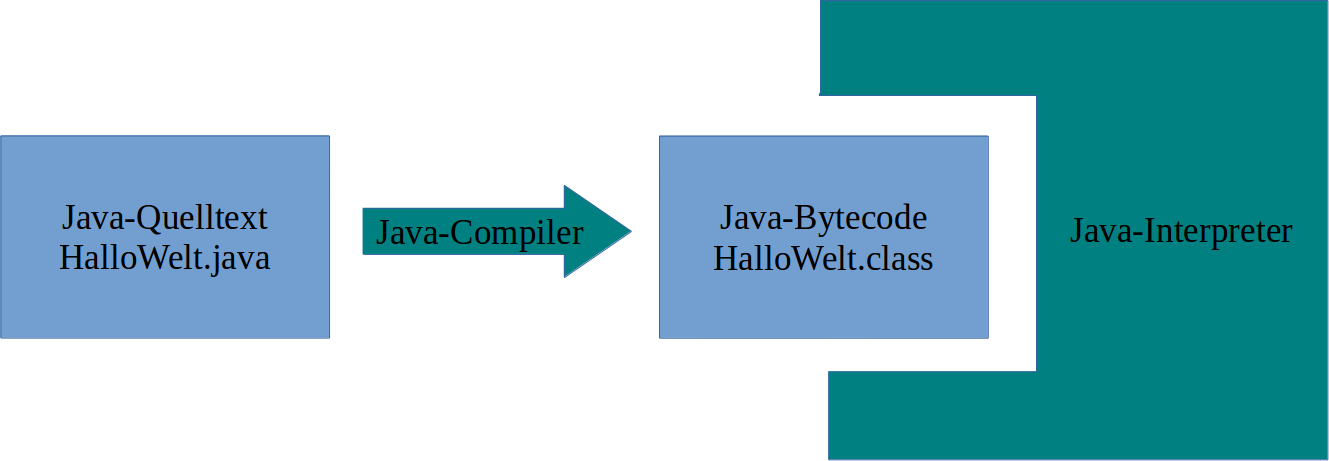
\includegraphics[width=0.8\textwidth]{grundl-java/Java-Kompiler}\\[2em]


\includegraphics[width=0.8\textwidth]{grundl-java/C++-Kompiler}

\begin{itemize}
 \item Java-Bytecode ist plattformunabhängig und kann vom Java-Interpreter auf jedem System ausgeführt werden.
 \item C++ Programme können direket vom Betriebssystem ausgeführt werden, wenn sie für dieses kompiliert wurden.
\end{itemize}

\end{frame}
